\documentclass{beamer}

\mode<presentation>
{
  \usetheme{Warsaw}       % or try default, Darmstadt, Warsaw, ...
  \usecolortheme{default} % or try albatross, beaver, crane, ...
  \usefonttheme{serif}    % or try default, structurebold, ...
  %\setbeamertemplate{navigation symbols}{}
  %\setbeamertemplate{caption}[numbered]
}


\usepackage[T1]{fontenc}
\usepackage[polish]{babel}
\usepackage[utf8]{inputenc}
\usetheme{default}


\title[Praca magisterska]{Zastosowanie analizy statycznej języka Ruby\\ w edytorach tekstu}
\author{Rafał Łasocha}
\institute{Promotor: prof. Witold Charatonik \\ Wydział Matematyki i Informatki \\ Instytut Informatyki}
\date{13 grudnia 2018}

\begin{document}

\begin{frame}
 \titlepage
\end{frame}
% programista Ruby na codzien
% znam problemy, brakuje narzedzia
% teraz powiem dlaczego taki temat

% dlaczego
\begin{frame}{Ruby}
 \begin{itemize}
  \item Interpretowany (interpreter i biblioteka standardowa w C)
  \item Dynamicznie typowany
  %\item Dynamic dispatch
  \item Zaawansowane mechanizmy obiektowe (wielokrotne dziedziczenie, klasy singletonowe)
  \item Metaprogramowanie (możliwość definiowania nowych klas, metod, zmiennych instancji, stałych w czasie działania programu)
  % Implikacja: juz na pierwszy rzut oka, analiza statyczna wydaje się być trudna
 \end{itemize}
\end{frame}

\begin{frame}{Pożądane funkcjonalności}
 \begin{itemize}
  \item Informacja o ``typie'' wyrażenia
  \item Skok do definicji klasy lub metody
  \item Autouzupełnianie dostępnych metod
  % pokazac ze sie sprowadza do znajomosci typu, screen some_object.push(42) i implikacja
  % Tu powiedzieć że dlatego właśnie wybrałem taki temat bo rozwiązanie nietrywialne
 \end{itemize}
\end{frame}

% co
\begin{frame}{Architektura projektu}
 \begin{itemize}
  \item Protokół komunikacji z edytorem tekstu (\textit{Language Server Protocol})
  \item Silnik dostarczający funkcjonalności niezależny od edytora
  \begin{figure}[htb]
    \centering
    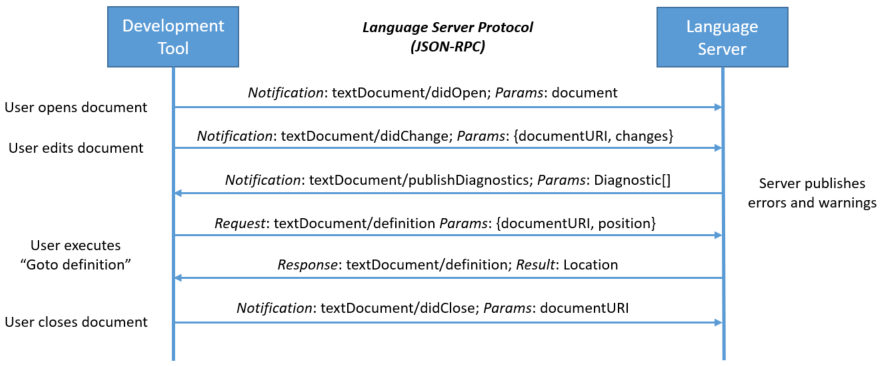
\includegraphics[scale=0.6]{lsp.png}
    {\tiny Źródło: https://microsoft.github.io/language-server-protocol/overview}
  \end{figure}
 \end{itemize}
\end{frame}


% jak
\begin{frame}{Zarys działania}
 \begin{enumerate}
  \item Parsowanie
  \item Budowanie grafu DFG (\textit{Data Flow Graph})
  \item Obliczenie typu dla każdego wierzchołka w grafie
 \end{enumerate}
\end{frame}

\begin{frame}{Zarys działania}
 \begin{block}{Parsowanie}
  Można skorzystać z gotowych rozwiązań.
 \end{block}
 \pause
 \begin{block}{Budowanie grafu DFG (\textit{Data Flow Graph})}
  Wymagane heurystyki, które obsłużą specjalne przypadki takie jak wywołania metod \texttt{private} czy \texttt{attr\_reader}.
 \end{block}
 \pause
 \begin{block}{Obliczenie typu dla każdego wierzchołka w grafie}
  Obliczenie typu wierzchołka $X$ korzysta z aktualnie obliczonych typów wierzchołków z krawędzią do $X$. Obsługa typów parametryzowanych takich jak \texttt{Array<Integer or String>}.
 \end{block}
\end{frame}

\begin{frame}{Przykład}
  \begin{figure}[htb]
    \centering
    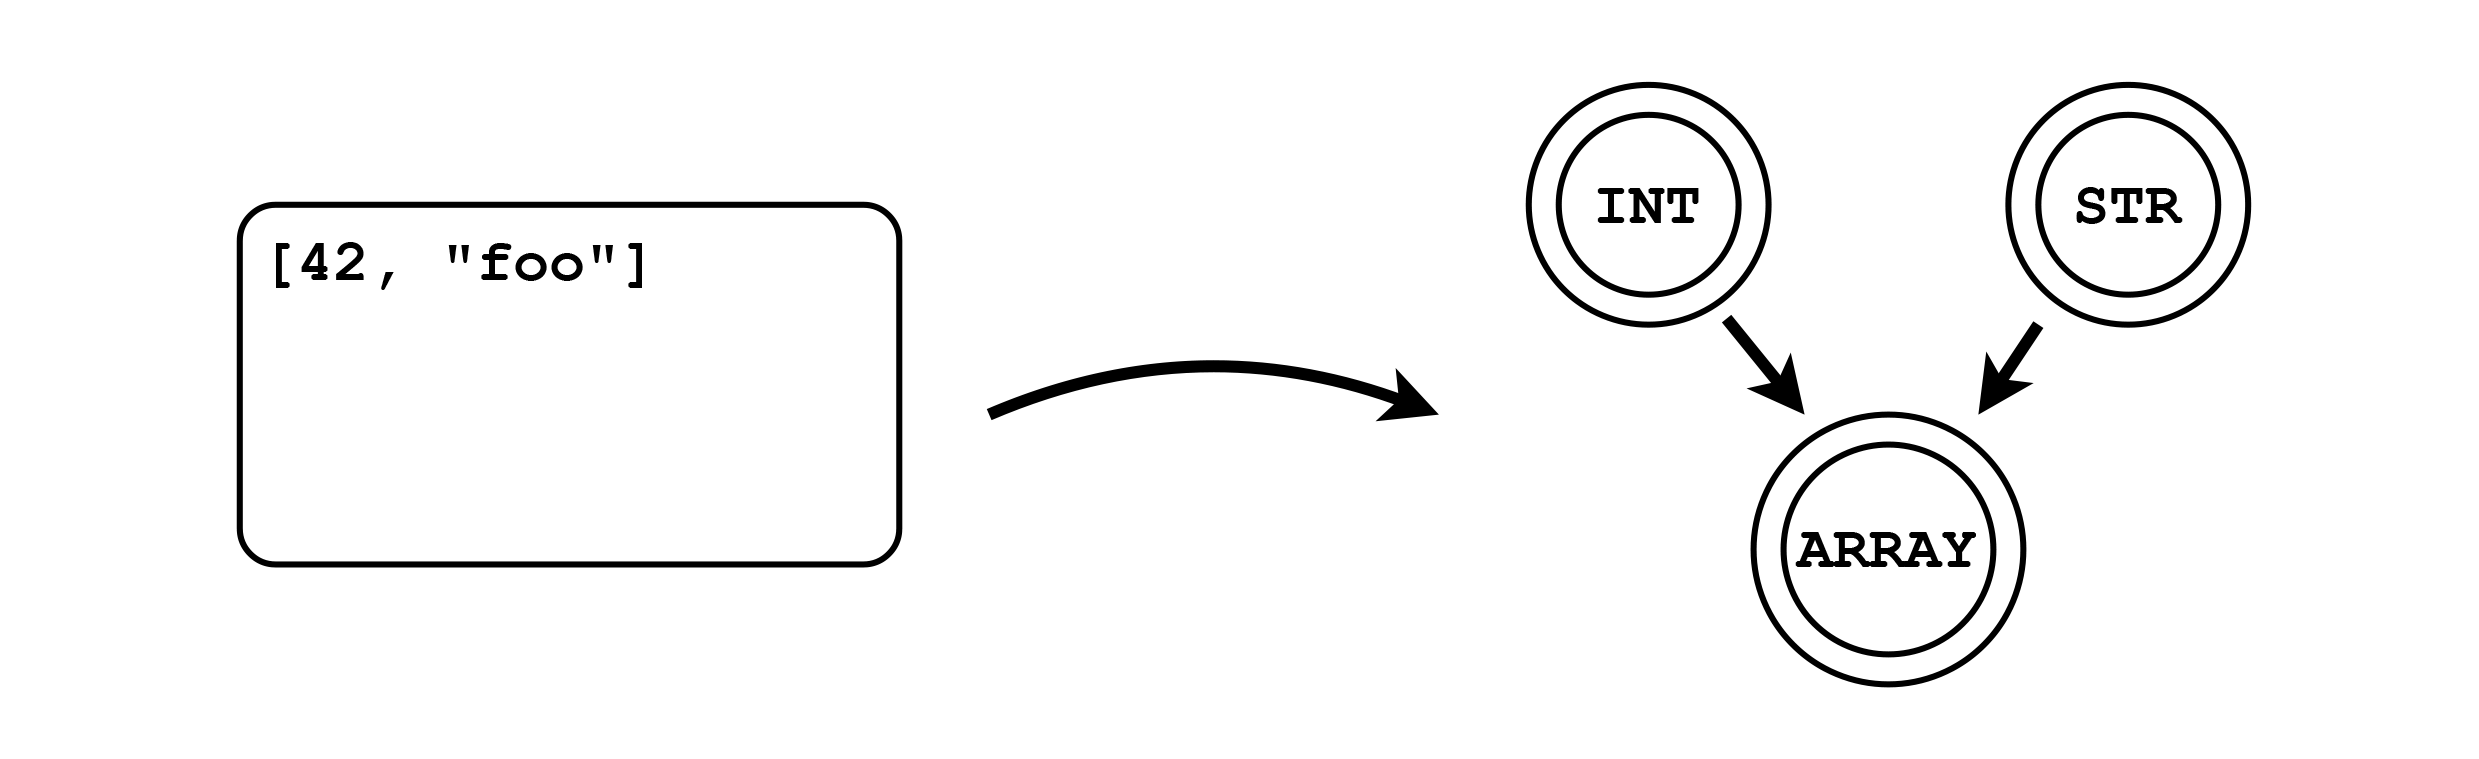
\includegraphics[scale=0.6]{msc-array.png}
  \end{figure}
\end{frame}

% parsowanie
% budujemy graf, kazde wyrazenie (ast) ma wierzcholek i sa dodatkowe; heurystyki odgrywaja istotna role bo public/private
% krawedz jezeli zalezy typ jednego wierzcholka zalezy od drugiego
% wnioskujemy typy
% prosty przyklad z array [42, 'foo']


% future
\begin{frame}{Możliwości rozwoju}
 \begin{itemize}
  \item obsługa metaprogramowania (w etapie zbierania definicji)
  % ["upcoming", "popular", "attending"].each do |event_kind|
  %define_method("#{event_kind}_events") do
  %  # rest of the code, possibly using `event_kind` variable
  %end
%end
  \item budowanie inkrementacyjne
 \end{itemize}
\end{frame}




\end{document}
